\documentclass[11pt]{article}
\usepackage{graphics}
\usepackage{amsthm}
\usepackage{amsmath}
\usepackage{amssymb}
\usepackage{bm}
\usepackage{amsbsy}
\usepackage{mathtools}
\usepackage{algpseudocode, algorithm, algorithmicx}
\usepackage{soul}
\usepackage{graphicx}
\usepackage{color}
\usepackage{float}
\usepackage{gensymb}
\usepackage{tabularx}
\newcommand{\ord}[1]{\textsuperscript{#1}}
\usepackage{ragged2e}
\DeclareMathOperator{\DICT}{DICT}


\graphicspath{ {images/HW5/} }

\makeatletter
\DeclareFontFamily{U}{tipa}{}
\DeclareFontShape{U}{tipa}{m}{n}{<->tipa10}{}
\newcommand{\arc@char}{{\usefont{U}{tipa}{m}{n}\symbol{62}}}%

\newcommand{\arc}[1]{\mathpalette\arc@arc{#1}}

\newcommand{\arc@arc}[2]{%
  \sbox0{$\m@th#1#2$}%
  \vbox{
    \hbox{\resizebox{\wd0}{\height}{\arc@char}}
    \nointerlineskip
    \box0
  }%
}
\makeatother

\makeatletter
\newcommand\multiline[1]{\parbox[t]{\dimexpr\linewidth-\ALG@thistlm}{#1}}
\makeatother
\usepackage[margin=1in]{geometry}
%\renewcommand{\baselinestretch}{1.2}
\newcommand{\codepar}[2]{\begin{minipage}[t]{#1}#2\end{minipage}}
\newcommand{\codecomt}[1]{\color{blue}\textit{// #1}\color{black}}

% You can put more user-defined commands here

\makeatletter
\newlength{\continueindent}
\setlength{\continueindent}{6em}

\renewenvironment{algorithmic}[1][0]%
   {%
   \edef\ALG@numberfreq{#1}%
   \def\@currentlabel{\theALG@line}%
   %
   \setcounter{ALG@line}{0}%
   \setcounter{ALG@rem}{0}%
   %
   \let\\\algbreak%
   %
   \expandafter\edef\csname ALG@currentblock@\theALG@nested\endcsname{0}%
   \expandafter\let\csname ALG@currentlifetime@\theALG@nested\endcsname\relax%
   %
   \begin{list}%
      {\ALG@step}%
      {%
      \rightmargin\z@%
      \itemsep\z@ \itemindent\z@ \listparindent2em%
      \partopsep\z@ \parskip\z@ \parsep\z@%
      \labelsep 0.5em \topsep 0.2em%\skip 1.2em 
      \ifthenelse{\equal{#1}{0}}%
         {\labelwidth 0.5em}%
         {\labelwidth 1.2em}%
       \leftmargin\labelwidth \addtolength{\leftmargin}{\labelsep}
      \ALG@tlm\z@%
      }%
      \parshape 2 \leftmargin \linewidth \continueindent \dimexpr\linewidth-\continueindent\relax
   \setcounter{ALG@nested}{0}%
   \ALG@beginalgorithmic%
   }%
   {% end{algorithmic}
   % check if all blocks are closed
   \ALG@closeloops%
   \expandafter\ifnum\csname ALG@currentblock@\theALG@nested\endcsname=0\relax%
   \else%
      \PackageError{algorithmicx}{Some blocks are not closed!!!}{}%
   \fi%
   \ALG@endalgorithmic%
   \end{list}%
   }%
\makeatother

\newcommand{\CH}{\mathrm{CH}}
\renewcommand{\thealgorithm}{}

\newenvironment{solution}
  {\renewcommand\qedsymbol{$\blacksquare$}\begin{proof}[Solution]}
  {\end{proof}}
  
 
\begin{document}

\hrule
\begin{center}
    \textbf{CS91T: Computational Geometry}\hfill \textbf{Fall 2023}\newline

    {\Large Homework 8}

    David Yang and Nick Fettig
\end{center}

\hrule

\vspace{1em}

\begin{enumerate}

\item\textbf{The dual $P^*$ of a point set $P$ is the set of all lines that are dual to points in $P$:}

\[P^* = \{p^*: p\in P\}\]

\textbf{What does the dual of the unit circle look like?}

\vspace{1em}

\begin{solution}

We claim that the dual of the unit circle is the region bounded above and below by the hyperbola $y^2-x^2 = 1.$ \\

\textbf{Lemma 1}. \textit{Any tangent line passing through a point on the hyperbola has a dual point on the unit circle.} \\

By definition, any point on the hyperbola must satisfy $y^2-x^2 = 1.$ By implicit differentiation, we find that
\[ 2y \, dy - 2x \, dx = 0\]

or equivalently, \[ \frac{dy}{dx} = \frac{x}{y}.\]

Since $y^2-x^2 = 1$, we can rewrite $x$ as $\pm \sqrt{y^2-1}.$ Substituting this into our above equation, we find that
\[ \frac{dy}{dx} = \frac{\pm \sqrt{y^2-1}}{y}.\]

Note that any point on the hyperbola must follow $|y| \geq 1$, so $y^2 - 1 \geq 0$ and $\sqrt{y^2-1} < \sqrt{y^2} = |y|.$ Thus, \[ \left|\frac{dy}{dx}\right| = \left|\frac{\pm \sqrt{y^2-1}}{y} \right| < 1.\]

Equivalently, the slope of the tangent line at any point on the parabola has a magnitude less than $1$, meaning its dual point in the dual plane will have $x$-coordinate between $-1$ and $1$ (note that the $x = \pm 1$ cases are properly handled due to the symmetries of the hyperbola about the $x$-axis). \\

It remains to show that the $y$-intercept of this tangent line passing through a point $(a,b)$ on the hyperbola is also between $-1$ and $1$. We know that the slope of the tangent line through $(a, b)$ is $\frac{dy}{dx} = \frac{a}{b}$ from our previous work, and $b^2 - a^2 = 1$ as $(a, b)$ lies on the hyperbola $y^2-x^2=1$. \\

Using point-slope form, we find that the equation of the tangent line through the point $(a, b)$ on the hyperbola is
\[ y - b = \frac{a}{b}(x-a). \]

Consequently, the $y$-intercept, which occurs when $x=0$, is \[ y = \frac{b^2-a^2}{b} = \frac{1}{b}.\]

Since $|b| \geq 1$, we know this intercept is between $-1$ and $1$. Furthermore, we find that the sum of the squares of the slope and intercept is $1$, as \[ \left(\frac{a}{b}\right)^2 + \left(\frac{1}{b}\right)^2 = \frac{a^2+1}{b^2} = 1\]

and so the tangent line through any point on the hyperbola has a corresponding dual point on the unit circle, as desired.

\textbf{Lemma 2}. \textit{Any point in the region bounded by the hyperbola lies on a tangent line passing through a point on the hyperbola.} \\

We will prove this claim with a geometric argument. Note that as our tangent lines spanning the first and third quadrants sweep towards those spanning the second and fourth quadrants, we sweep across every point in the interior of this bounded region. Thus, with this sweeping argument, we see that any point in the region bounded by the hyperbola lies on a tangent line passing through a point on the hyperbola. \\

By Lemma 1, we know that the dual of a point on the unit circle corresponds to a tangent line passing through a point on the hyperbola $y^2-x^2 = 1$. Furthermore, by Lemma 2, any point in the region bounded by this hyperbola from above and below must lie on one of these tangent lines. Thus, the dual of the unit circle is the region bounded above and below by the hyperbola $y^2-x^2 = 1$, as desired. \\

\begin{center}
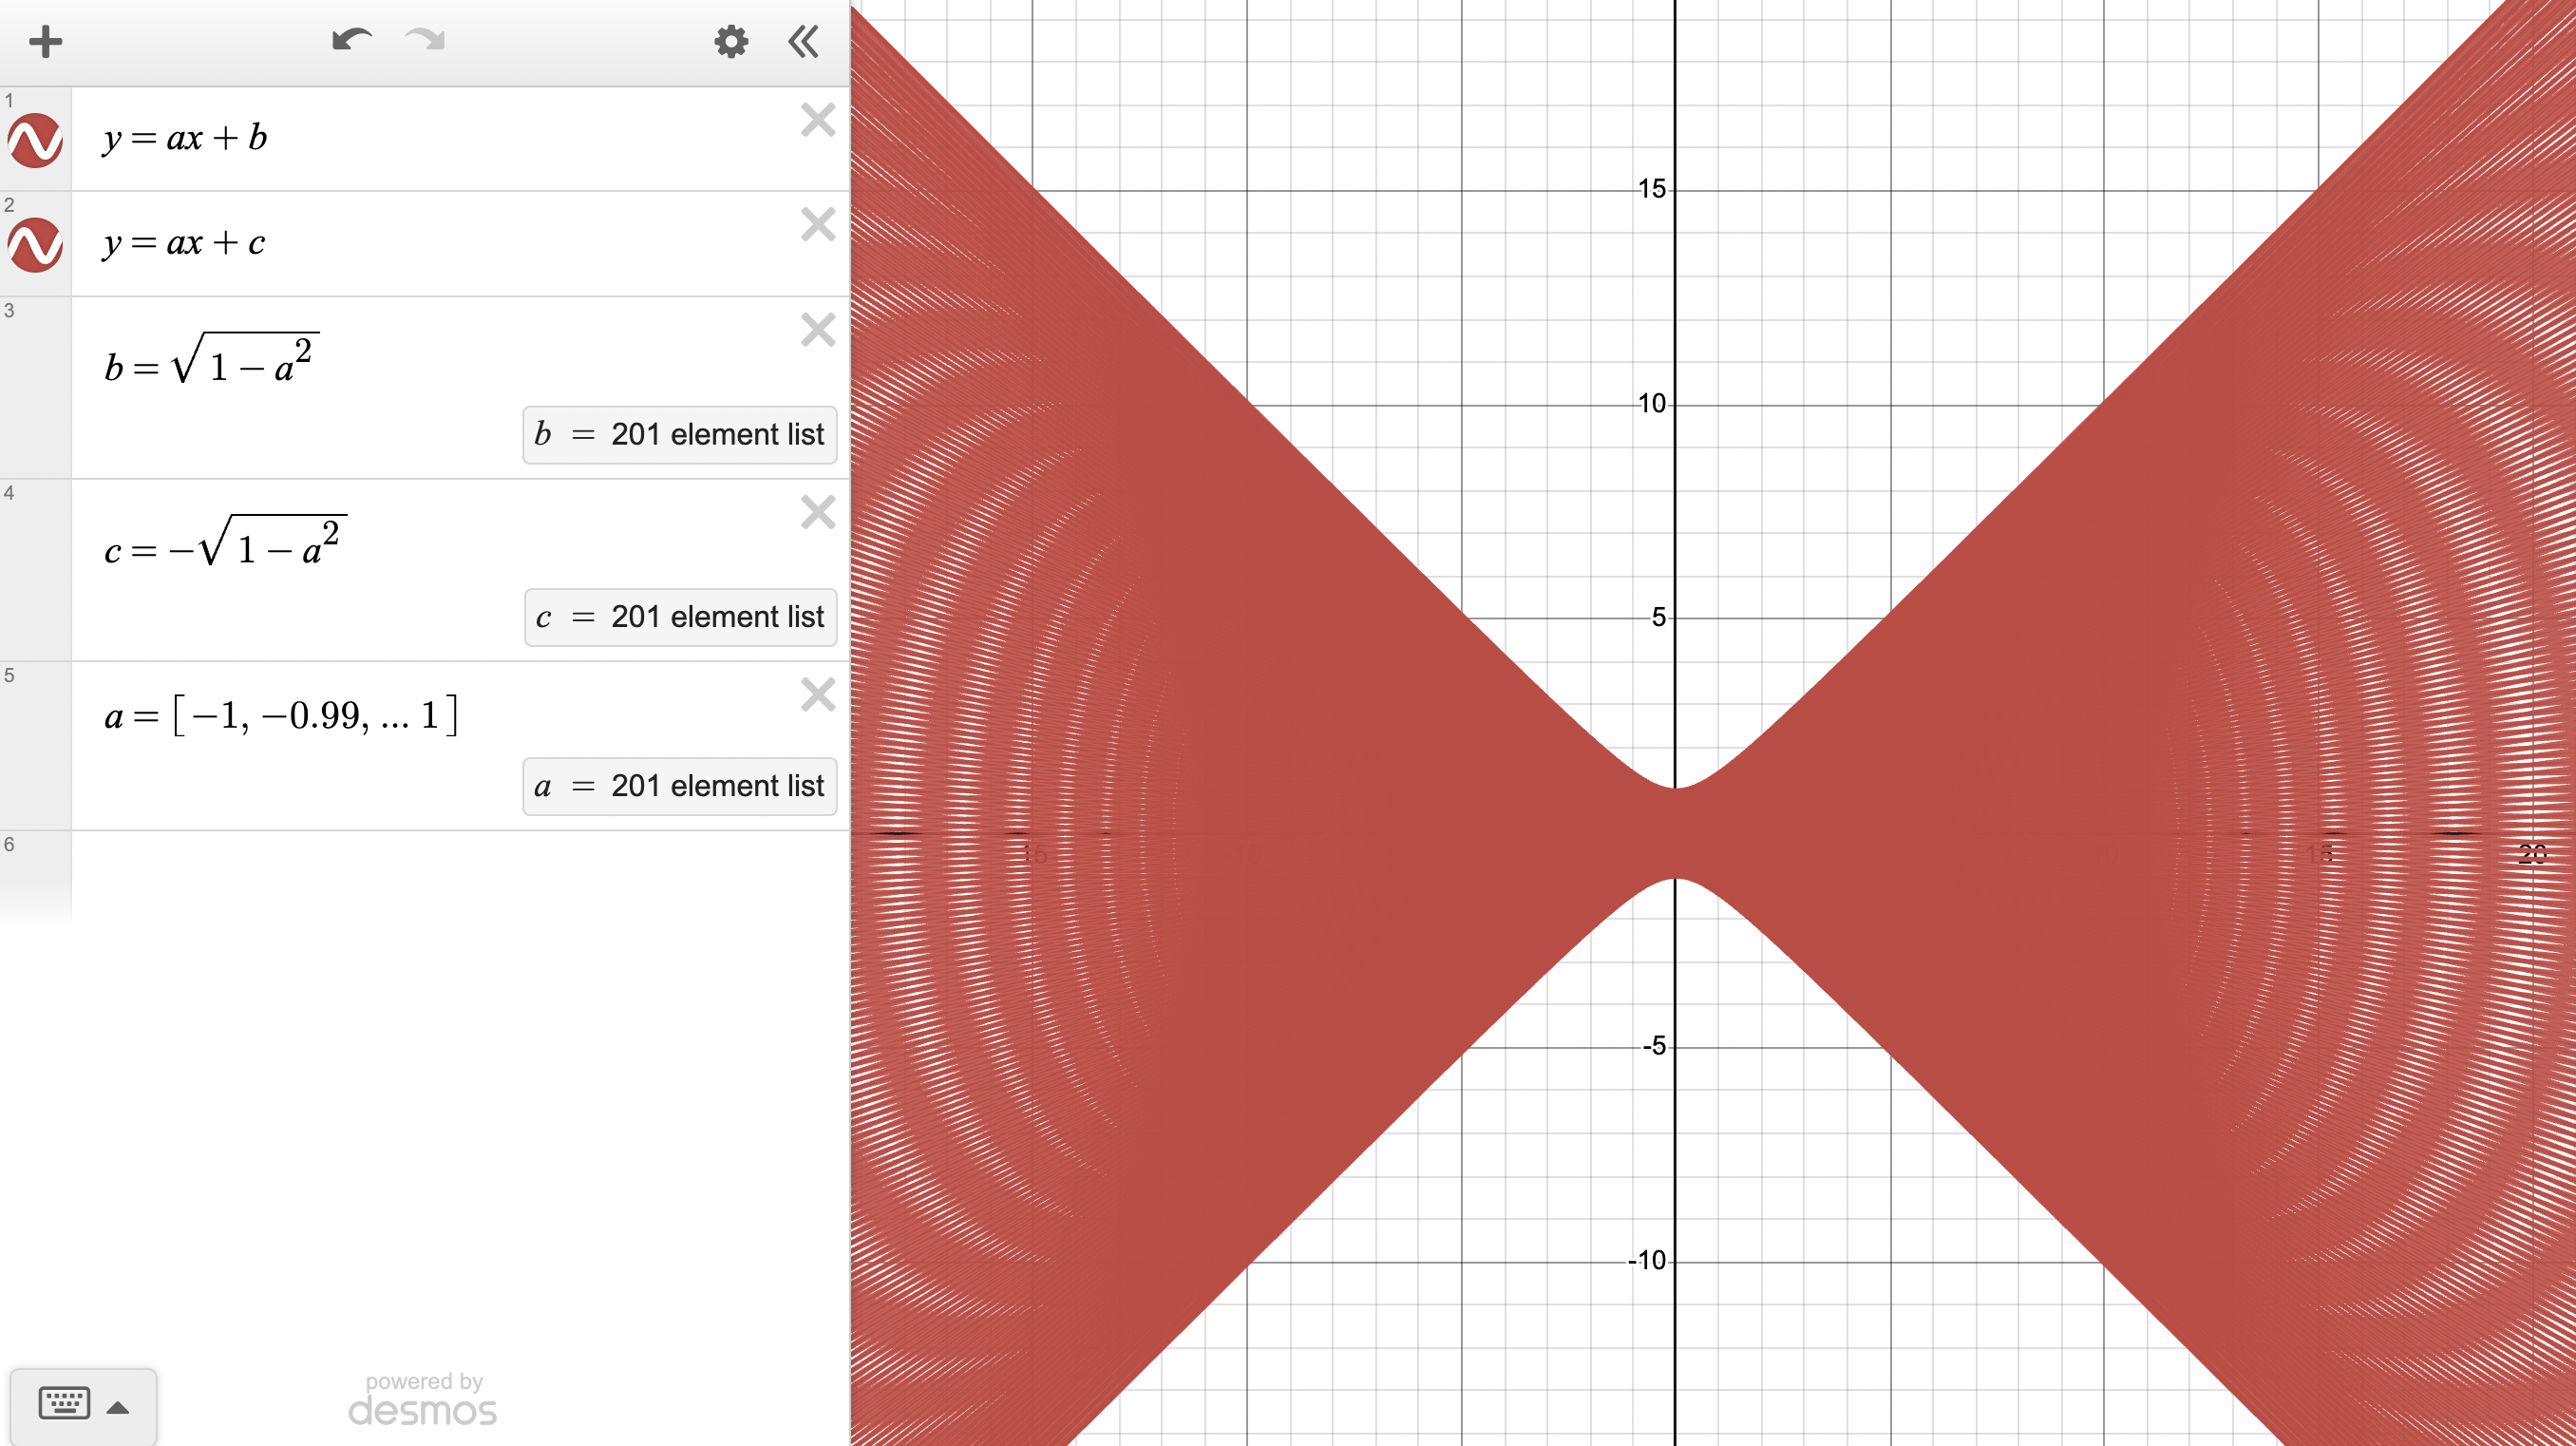
\includegraphics[scale=0.2]{images/HW8/part_1_desmos.png}
\end{center}

\end{solution}

\newpage 

\item\textbf{Let $P$ be a set of $n$ points in the plane, and let $p\in P$. Prove that $p$ lies on the lower hull of $P$ if and only if the line $p^*$ is visible from above in the line set $P^* = \{q^*: q \in P\}$.}

\begin{solution}

Note that by convexity of the convex hull, a point lies on the lower hull of $P$ if and only if there is a line through it such that every other point is above that line. \\

Similarly, for a dual line $p^*$ to be visible from above, there must be a point on that line such that no line in the line set $P^*$ lies above it. These statements are equivalent statements, given the duality of the points in $P$ with the dual line set $P^*$, and a line in $P$ with the dual point on $p^*$. \\

Consequently, a point $p$ lies on the lower hull of $P$ if and only if the line $p^*$ is visible from above in the line set $P^*$, as desired.\end{solution}


\newpage

\item\textbf{Let $P$ be a set of $n$ points in the plane, and let $p \in P$. Give an expected O($n$)-time randomized algorithm for determining whether $p$ lies on the boundary of CH($P$).}

Given a set $P$ of $n$ points in the plane and a point $p$ to determine whether $p$ is on the boundary of CH($P$), we define the algorithm \textsc{OnCHBoundary}($P$, $p$) as follows:
\begin{enumerate}
    \item Find the dual graph $P^*$ of the point set $P \setminus p$.
    \item Create two linear programs, \textsc{LP\_\,above} and \textsc{LP\_\,below}, using the equations of the lines of $P^*$ with:
        \begin{itemize}
        \item trivial optimization function (constant).
        \item for each line $\ell$ in $P^*$, a linear constraint for \textsc{LP\_\,above} defined by the half-plane above $\ell$
        \item for each line $\ell$ in $P^*$, a linear constraint for \textsc{LP\_\,below} defined by the half-plane below $\ell$
        \item for the dual line $p^*$ of $p$, two linear constraints, defined by the half-planes that include/lie above and include/lie below $p^*$.
        \end{itemize}
    \item Randomize the constraints of \textsc{LP\_\,above} and \textsc{LP\_\,below}
    \item Run the linear programs \textsc{LP\_\,above} and \textsc{LP\_\,below}.
    \item Store the results of the feasible regions to the two linear programs in \textsc{FR\_\,above} and \textsc{FR\_\,below}, as a clockwise list of points (if they exist)
    \item Use the lists \textsc{FR\_\,above} and \textsc{FR\_\,below} to determine whether $p^*$ is visible from above or below in the line set $P^*$
    \item If it is, \textbf{return True}. Otherwise, \textbf{return False}.
\end{enumerate}

\textbf{Runtime Analysis}: Finding the dual graph in step (a) can be done in $O(n)$ time. Creating the two linear programs in step (b) can also be done in linear time; for each linear program, we require constant time to set up each of the $O(n)$ constraints. Randomizing the constraints in step (c) and running the linear program in step (d) takes $O(n)$ expected time, as per our previous analysis. Determining and storing the feasible region in step (e) takes linear time. Finally, step (f) can also be completed in at most linear time. \\

Thus, our algorithm is an $O(n)$ expected time randomized algorithm, as desired. \\

\textbf{Proof of Correctness}: Our randomized algorithm relies on problem 2; we know that $p$ lies on the lower hull of $P$ if and only if the line $p^*$ is visible from above in the line set. \\

Setting up our linear programs \textsc{LP\_\,above} and \textsc{LP\_\,below} helps us determine the relevant feasible regions \textsc{FR\_\,above} and \textsc{FR\_\,below}. The points in each feasible region correspond to intersections between our dual line and dual lines in $P^*$. Finally, by our result from problem 2, checking whether $p^*$ is visible from above or below in the line set $P^*$ is an equivalent condition for determining whether $p$ is on the upper or lower hull of CH($P$). \\

Thus, our randomized algorithm works as desired, finding whether $p$ lies on the boundary of CH($P$).


\newpage

\item\textbf{Suppose you have $n$ vertical segments in the plane, and you want to find a single line that intersects all of these segments, if such a line exists. Design an expected O($n$)-time randomized algorithm for this task.}

Given a set $S$ of $n$ vertical segments, we define the algorithm \textsc{LVSI} (\textsc{Line-Vertical Segment Intersection}) as follows:
\begin{enumerate}
    \item Initialize $P$ to be an empty list
    \item For each of the $n$ segments in $S$, add each endpoint to $P$ along with an indicator for whether that point was the upper or lower point in the vertical segment
    \item Find the dual graph $P^*$ of the point set $P$.
    \item Create a linear program \textsc{LP} using the equations of the lines of $P^*$ with:
        \begin{itemize}
        \item trivial optimization function (constant).
        \item for each line $\ell$ in $P^*$ corresponding to an upper endpoint in $P$, the linear constraint defined by the half-plane under $\ell$  \item for each line $\ell$ in $P^*$ corresponding to an upper endpoint in $P$, the linear constraint defined by the half-plane above $\ell$  
        \end{itemize}
    \item Randomize the constraints of LP
    \item Run LP and determine the feasible region
    \item If a feasible region exists, take any point in the feasible region. Find the line that is the dual of this point, and return it.
\end{enumerate}

\textbf{Runtime Analysis}: Steps (a) to (c) constitute the initialization phase of our algorithm. Steps (b) and (c) can each be done in $O(n)$ time. Creating the linear program in step (d) can also be done in linear time; we require constant time to set up each of the $O(n)$ constraints. Randomizing the constraints in step (e) and running the linear program in step (f) takes $O(n)$ expected time, as per our previous analysis. Finally, determining the feasible region and finding a given line (if it exists) in steps (f) and (g) take linear time, at most. \\

Thus, our algorithm is an $O(n)$ expected time randomized algorithm, as desired. \\

\textbf{Proof of Correctness}: Our randomized algorithm relies on the fact that a line intersects each of the $n$ vertical segments if and only if, after converting every endpoint of a segment to a line in the dual plane, there is a point in the feasible region of a linear program bounded by the dual lines. \\

Consider one such vertical segment $s$ from $(a, b)$ to $(a, c)$. A line $\ell$ intersects this segment at some point $(a, d)$ with $d \in [b, c]$ if and only if $ax - b \leq d \leq ax-c$. Equivalently, the point corresponding to $\ell$ in the dual plane must lie between (or on) the lines $ax-b$ and $ax-c$, which are the dual lines of the endpoints of the segment $s$. \\

If there is a point in the feasible region of a linear program defined by the dual lines of the endpoints of our initial $n$ vertical segments, then its dual is a line that intersects all of these segments. Thus, our randomized algorithm works as desired, to find a line that intersects each of the $n$ vertical segments, if it exists.

\end{enumerate}
\end{document}